\documentclass[draft, twocolumn]{article}
\usepackage[unicode,draft=false,hidelinks]{hyperref}
\usepackage{cite}
\usepackage{catchfilebetweentags}
\usepackage{amssymb}
\usepackage{turnstile}
\usepackage{bbm}
\usepackage[greek, english]{babel}
\usepackage{MnSymbol}
\usepackage{stmaryrd}
\usepackage{csquotes}
\newcommand\doubleplus{+\kern-1.3ex+\kern0.8ex}
\newcommand\mdoubleplus{\ensuremath{\mathbin{+\mkern-8mu+}}}
\makeatletter
\newcommand\incircbin
{%
  \mathpalette\@incircbin
}
\newcommand\@incircbin[2]
{%
  \mathbin%
  {%
    \ooalign{\hidewidth$#1#2$\hidewidth\crcr$#1\bigcirc$}%
  }%
}
\newcommand{\oeq}{\ensuremath{\incircbin{=}}}
\makeatother
\usepackage{ucs}
\DeclareUnicodeCharacter{8759}{\ensuremath{\squaredots}}
\DeclareUnicodeCharacter{951}{\textgreek{\texteta}}
\DeclareUnicodeCharacter{737}{\ensuremath{^\text{l}}}
\DeclareUnicodeCharacter{691}{\ensuremath{^\text{r}}}
\DeclareUnicodeCharacter{7523}{\ensuremath{_\text{r}}}
\DeclareUnicodeCharacter{8718}{\ensuremath{\blacksquare}}
\DeclareUnicodeCharacter{957}{\textgreek{\textnu}}
\DeclareUnicodeCharacter{961}{\textgreek{\textrho}}
\DeclareUnicodeCharacter{929}{\textgreek{\textRho}}
\DeclareUnicodeCharacter{954}{\textgreek{\textkappa}}
\DeclareUnicodeCharacter{10214}{\ensuremath{\lsem}}
\DeclareUnicodeCharacter{10215}{\ensuremath{\rsem}}
\DeclareUnicodeCharacter{8857}{\mdoubleplus}
\DeclareUnicodeCharacter{8860}{\oeq}
\DeclareUnicodeCharacter{9043}{\ensuremath{\triangle}}
\DeclareUnicodeCharacter{928}{\textgreek{\textPi}}
\DeclareUnicodeCharacter{922}{\textgreek{\textKappa}}
\DeclareUnicodeCharacter{931}{\textgreek{\textSigma}}
\DeclareUnicodeCharacter{916}{\textgreek{\textDelta}}
\DeclareUnicodeCharacter{8779}{\ensuremath{\backtriplesim}}
\DeclareUnicodeCharacter{8799}{\ensuremath{\stackrel{?}{=}}}
\DeclareUnicodeCharacter{10181}{\ensuremath{\lbag}}
\DeclareUnicodeCharacter{10182}{\ensuremath{\rbag}}
\usepackage[utf8x]{inputenc}
\usepackage[T1]{fontenc}
\usepackage{autofe}
\usepackage[references]{agda}
\usepackage{bbding}
\setlength{\marginparwidth}{2cm}
\usepackage[obeyDraft]{todonotes}
\usepackage{lineno}
\setlength\linenumbersep{-0.5cm}
\usepackage{amsthm}
\theoremstyle{definition}
\newtheorem{definition}{Definition}[section]
\theoremstyle{remark}
\newtheorem{principle}{Principle}[section]
\usepackage{subcaption}
\usepackage{graphicx}
\usepackage{tikz}
\usetikzlibrary{decorations.pathmorphing}
\usetikzlibrary{snakes}
\usetikzlibrary{arrows}
\usetikzlibrary{cd}
\usepackage{forest}
\author{Donnacha Oisín Kidney}
\title{An Efficient and Flexible Evidence-Providing Polynomial Solver in Agda}
\begin{document}
\maketitle
\begin{abstract}
  We present a new implementation of a ring solver in the programming language
  Agda\cite{norell_dependently_2008}. The new implementation is significantly
  more efficient than the version in the standard
  library\cite{danielsson_agda_2018}, bringing it in line with Coq's \verb+ring+
  tactic\cite{the_coq_development_team_2018_1219885},
  \cite{hutchison_proving_2005}. 

  We demonstrate techniques for constructing proofs based on the theory of
  lists, show how Agda's reflection system can be used to provide a safe and
  simple interface to the solver, and compare the ``correct by construction''
  approach to that of auxiliary proofs.
  
  We also show that, as a by-product of proving equivalences rather than
  equalities, the prover can be used to provide artifacts other than equational
  proofs, including step-by-step solutions, and isomorphisms.
\end{abstract}
\tableofcontents
\section{Introduction}
Dependently typed programming languages allow programmers and mathematicians
alike to write proofs which can be executed. For programmers, this often means
being able to formally verify the properties of their programs; for
mathematicians, it provides a system for writing machine-checked (rather than
hand-checked) proofs.

Naïve usage of these systems can be tedious: the typechecker is often
over-zealous in its rigor, demanding justification for every minute step in a
proof, no matter how obvious or trivial it may seem to a human. For algebraic
proofs, this kind of thing usually consists of long chains of rewrites, of the
style ``apply commutativity of \(+\), then associativity of \(+\), then at this
position apply distributivity of \(*\) over \(+\)'' and so on, when really the
programmer wants to say ``rearrange the expression into this form, checking it's
correct''.

However, since our proof assistant is also a programming language, we can
automate this process by writing a verified program to compute these proofs for
us. 
\section{A Case Study in Monoids}
Before describing the ring solver, first we will explain the technique of
writing a solver in Agda in the simpler setting of monoids.

\begin{definition}{Monoids}
  A monoid is a set equipped with a binary operation, \(\bullet\), and a
  distinguished element \(\epsilon\), such that the following equations hold:
  \begin{align}
    x \bullet (y \bullet z) &= (x \bullet y) \bullet z \tag{Associativity} \\
    x \bullet \epsilon      &= x \tag{Left Identity} \\
    \epsilon \bullet x      &= x \tag{Right Identity}
  \end{align}
\end{definition}
Addition and multiplication (with 0 and 1 being the respective identity
elements) are perhaps the most obvious instances of the algebra. In computer
science, monoids have proved a useful abstraction for formalizing concurrency
(in a sense, an associative operator is one which can be evaluated in any
order).

Monoids can be represented in Agda in a straightforward way, as a record (see
Figure~\ref{mon-def}). Immediately it should be noted that we're no longer
talking about a monoid over a set, but rather one over a setoid. In other words,
rather than using propositional equality (indicated by the \(\AgdaDatatype{≡}\)
symbol), we will use a user-supplied equivalence relation (\(\AgdaField{≈}\) in
Figure~\ref{mon-def}) in our proofs.
\begin{figure}
  \ExecuteMetaData[Monoids.tex]{mon-def}
  \caption{The definition of Monoid in the Agda Standard
    Library\cite{danielsson_agda_2018}}
  \label{mon-def}
\end{figure}
\subsection{Equivalence Proofs}
Propositions are stated in type signatures in dependently typed languages.
Figure~\ref{mon-ident} is an example of such a proposition.
\begin{figure}[h]
  \ExecuteMetaData[Monoids.tex]{mon-ident}
  \caption{Example Identity}
  \label{mon-ident}
\end{figure}
To a human, the fact that the identity holds may well be obvious:
\(\AgdaField{∙}\) is associative, so we can scrub out all the parentheses, and
\(\AgdaField{ε}\) is the identity element, so scrub it out too. After that, both
sides are equal, so voilà!

Unfortunately, to convince the compiler we need to specify every instance of
associativity and identity, rewriting the left-hand-side repeatedly until it
matches the right:

\begin{samepage}
  \begin{linenumbers}
    \ExecuteMetaData[Monoids.tex]{mon-proof}
  \end{linenumbers}
\end{samepage}

The syntax is designed to mimic that of a handwritten proof: line 3 is the
expression on the left-hand side of \(\AgdaField{≈}\) in the type, and line 9
the right-hand-side. In between, the expression is repeatedly rewritten into
equivalent forms, with justification provided inside the angle brackets. For
instance, to translate the expression from the form on line 3 to that on line 5,
the associative property of \(\AgdaField{∙}\) is used on line 4.

Because we're not using propositional equality, some familiar tools are
unavailable, like Agda's rewrite mechanism, or function congruence (this is why
we have to explicitly specify the congruence we're using on line 6). The purpose
of this particular hair shirt is flexibility: users can still use the solver
even if their type only satisfies the monoid laws modulo some equivalence
relation (perhaps they are have an implementation of finite, mergeable sets as
balanced trees, and want to treat two sets as equivalent if their elements are
equal, even if their internal structures are not). Beyond flexibility, we get
some other interesting applications, which are explored in
section~\ref{setoid-applications}.

Despite the pleasant syntax, the proof is mechanical, and it's clear that
similar proofs would become tedious with more variables or more complex algebras
(like rings). To avoid the tedium, then, we automate the procedure.
\subsection{Canonical Forms}
Automation of equality proofs like the one above can be accomplished by first
rewriting both sides of the equation into a canonical form. Not every algebra
has a canonical form: monoids do, though, and it's the simple list.
\ExecuteMetaData[Monoids.tex]{list-def}
We're going to treat this type like an AST for a simple ``language of lists''.
This language supports two functions: the empty list, and concatenation.
\ExecuteMetaData[Monoids.tex]{list-monoid}
The type itself parameterized by the number of variables it contains. Users can
refer to variables by their index:
\ExecuteMetaData[Monoids.tex]{list-vars}
And we can interpret this language with values for each variable supplied in a
vector:
\ExecuteMetaData[Monoids.tex]{list-eval}

Compare this language to the language of monoid expressions that
Figure~\ref{mon-ident} uses: both have identity elements and a binary operator,
and both refer to variables. Our language of lists, however, has one significant
advantage: the monoid operations don't depend on the contents of the lists, only
the structure. In other words, an expression in the language of lists will
reduce to a flat list even if it has elements which are abstract variables. As a
result, the identity from Figure~\ref{mon-ident} is \emph{definitionally} true
when written in the language of lists:
\ExecuteMetaData[Monoids.tex]{list-obvious}
\subsection{Extracting Evidence}
While this is beginning to look like a solver, it's still not entirely clear how
we're going to join up the pieces. The first step is to get a concrete
representation of expressions which we can manipulate and pattern-match on
(Figure~\ref{mon-ast}).
\begin{figure}[h]
  \ExecuteMetaData[Monoids.tex]{mon-ast}
  \caption{The AST for monoid expressions}
  \label{mon-ast}
\end{figure}
It has constructors for each of the monoid operations
(\(\AgdaInductiveConstructor{⊕}\) and \(\AgdaInductiveConstructor{e}\) are
\(\AgdaField{∙}\) and \(\AgdaField{ε}\), respectively), and it's indexed by the
number of variables it contains, which are constructed with
\(\AgdaInductiveConstructor{ν}\).

We can convert from this AST to an unnormalized expression like so\footnotemark:
\ExecuteMetaData[Monoids.tex]{eval-ast}
Because this function performs no normalization or transformation, the output is
definitionally equal to its equivalent expression. This means that we can
discharge the proof obligation with \(\AgdaFunction{refl}\):
\footnotetext{
  The type of the unnormalized expression has changed slightly: instead of being
  a curried function of \(n\) arguments, it's now a function which takes a
  vector of length \(n\). The final solver has an extra translation step for
  going between these two representations, but it's a little fiddly, and not
  directly relevant to what we're doing here, so we've glossed over it. We refer
  the interested reader to the Relation.Binary.Reflection module of Agda's
  standard library\cite{danielsson_agda_2018} for an implementation.
}
\ExecuteMetaData[Monoids.tex]{eval-nonnorm}

The AST might look ugly, but it gives us a link between the expressions we had
in Figure~\ref{mon-ident} and a concrete representation. The next link is
between the AST and the normalized expression. We can convert from the AST to a
normal form like so:
\ExecuteMetaData[Monoids.tex]{ast-norm}
And since we already defined how to ``evaluate'' the list normal form, we can
combine both steps into one:
\ExecuteMetaData[Monoids.tex]{ast-norm-interp}

Now we have a concrete way to link the normalized and non-normalized forms of
the expressions. A diagram of the strategy for constructing our proof is in
Figure~\ref{proof-process}. The goal is to construct a proof of equivalence
between the two expressions at the bottom: to do this, we first construct the
AST which represents the two expressions (for now, we'll assume the user
constructs this AST themselves. Later we'll see how too construct it
automatically from the provided expressions). Then, we can evaluate it into
either the normalized form, or the unnormalized form. Since the normalized forms
are syntactically equal, all we need is \(\AgdaInductiveConstructor{refl}\) to
prove their equality. The only missing part now is \(\AgdaFunction{correct}\),
which is the task of the next section.

\begin{figure*}
  \makebox[\textwidth][c]{
    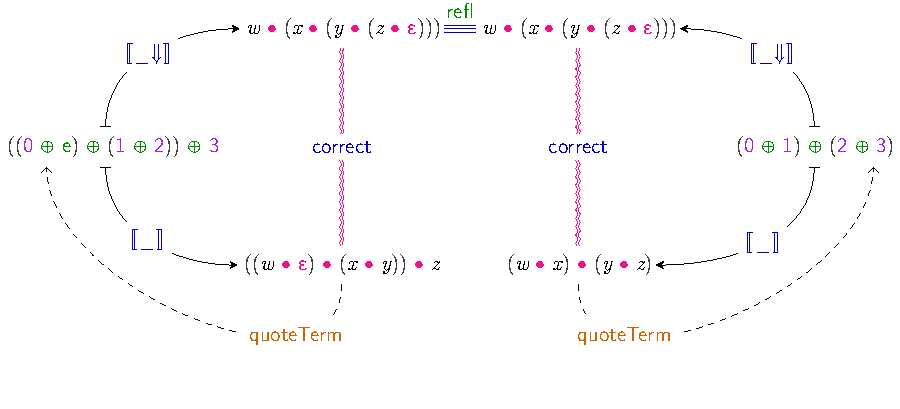
\includegraphics[draft=false]{graphics/reflexive-process};
    }
  \caption{The Reflexive Proof Process}
  \label{proof-process}
\end{figure*}
\bibliographystyle{IEEEtranS}
\bibliography{bibliography.bib}
\end{document}